En esta sección se detalla la implementación de cada paso realizado para el preprocesamiento de los datos, el cual se lleva a cabo después de la fase de limpieza de texto. En esta etapa, se trabaja con documentos de texto ya despojados de su formato original, facilitando su segmentación y tratamiento posterior. El objetivo principal del preprocesamiento es manejar la estructura interna del texto, segmentándolo en frases, oraciones o palabras, según sea más conveniente. El resultado de este proceso es un conjunto de datos limpio, útil y en uno de los formatos estándar aceptables para el uso del modelo de etiquetado. A continuación, se describe el archivo encargado del preprocesamiento de comentarios:

\begin{itemize}

\item corrector\_lenguaje.py: Este archivo aborda los aspectos generales de limpieza que se aplican a cualquier tipo de información, independientemente de su fuente. Los detalles de este archivo se muestran en la figura \ref{fig:uml2}.

\begin{figure}
	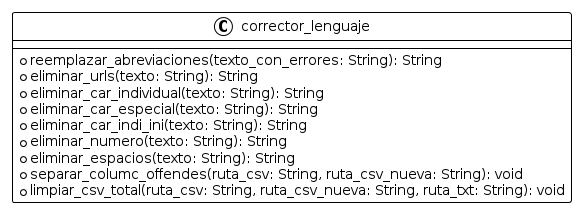
\includegraphics[width=0.65\textwidth]{capitulo5/figuras/fig2.png}
	\caption{Diagrama de clase del archivo corrector\_lenguaje}
	\floatfoot{Fuente: Elaboración propia, generado con PlantUML}
	\label{fig:uml2}
\end{figure}

\end{itemize}

La carpeta gestionarchivos contiene el archivo limpiar\_datos.py, que es utilizado en convertir\_formato.py. De manera similar, corrector\_lenguaje.py emplea el archivo manejo\_archivos.py, también ubicado en la misma carpeta. Esta organización permite que ambos archivos compartan la carpeta para aprovechar las funciones de tratamiento de formatos y la manipulación masiva de datos en múltiples archivos.
Una vez que los datos han pasado por los procesos de limpieza y preprocesamiento, se obtiene un producto final listo para ser utilizado en modelos de aprendizaje.


